%\documentclass[11pt,a4paper,uplatex,dvipdfmx]{ujarticle} 		% for uplatex
\documentclass[11pt,a4j,dvipdfmx]{jarticle} 					% for platex
%=======================================
% form00_header.tex
%	General header for kakenhiLaTeX,  Moved over from form00_2010_header.tex.
%	2009-09-06 Taku Yamanaka (Osaka Univ.)
%==== General Version History ======================================
% 2006-05-30 Taku Yamanaka (Physics Dept., Osaka Univ.)
% 2006-06-02 V1.0
% 2006-06-14 V1.1 Use automatic calculation for cost tables.
% 2006-06-18 V1.2 Split user's contents and the format.
% 2006-06-20 V1.3 Reorganized user and format files
% 2006-06-25 V1.4 Readjusted all the table column widths with p{...}.
%				With \KLTabR and \KLTabRNum, now the items can be right-justified
%				in the cell defined by p{...}.
% 2006-06-26 V1.5 Use \newlength and \setlength, instead of \newcommand, to define positions.
% 2006-08-19 V1.6 Remade it for 2007 JFY version.
% 2006-09-05 V1.7 Added font declarations suggested by Hoshino@Meisei Univ.
% 2006-09-06 V1.8 Introduced usePDFform flag to switch the form file format.
% 2006-09-09 V1.9 Changed p.7, to allow different heights between years. (Thanks to Ytow.)
% 2006-09-11 V2.0 Added an option to show budget summary.
% 2006-09-13 V2.1 Added an option to show the group.
% 2006-09-14 V2.1.1 Cleaned up Kenkyush Chosho.
% 2006-09-21 V2.2 Generated under a new automatic development system.

% 2007-03-24 V3.0 Switched to a method using "picture" environment.

% 2007-08-14 V3.1 Switched to kakenhi3.sty.
% 2007-09-17 V3.2 Added \KLMaxYearCount
% 2008-03-08 V3.3 Remade it for 2009 JFY version\
% 2008-09-08 V3.4 Added \KLXf ... \KLXh.
% 2011-10-20 V5.0 Use kakenhi5.sty, to utilize array package in tabular environment.
% 2012-08-14 v5.1 Moved preamble and kakenhi5 into the current directory, instead of the parent directory.
% 2012-11-10 v6.0 Switched to kakenhi6.sty.
% 2015-08-26 v6.1 Added KLFirstPageIsLongPage flag.
% 2017-05-27 v7.0 Simplified for the new format.
%=======================================
% Dummy section and subsection commands.
% With these, some editors (such as TeXShop, etc.) can jump to the (sub)sections.
\newcommand{\dummy}{dummy}% 
\renewcommand{\section}[1]{\renewcommand{\dummy}{#1}}

\usepackage{calc}
\usepackage{geometry}                % See geometry.pdf to learn the layout options. There are lots.
\usepackage[dvipdfmx]{graphicx}
\usepackage{color}
\usepackage{ifthen}
\usepackage{udline}
\usepackage{array}
\usepackage{longtable}
\usepackage{fancyhdr}
 % pieces
%==================================================
% kakenhi7.sty
%==================================================
% v1
% Minimum amount of macros for writing Kakenhi forms.
%
% 2005-10-24 Taku Yamanaka, Physics Dept. Osaka Univ.
%		taku@hep.sci.osaka-u.ac.jp
% 		Macros such as XYBC, etc. were imported from Kakenhi Macro at
% 		http://www.yukawa.kyoto-u.ac.jp/contents/researcher/kakenhi.html .
% 2006-06-04 Taku
%		Added macros to draw boxes if \DrawBox is in the source.
%		This is useful when designing the LaTeX forms.
% 2006-06-14 Taku
%		Added LaTeX macros to add costs 
%		(\KLResetGrandSum, \KLCostItem, \KLSum, \KLGrandSum).
%		Added a macro \Number to supply commas every 3 digits (imported from kkh.mac).
% 2006-06-25 Taku
%		Added \KLTabC, \KLTabR, \KLTabRNum to specify alignments in tables.
%		Please note that \phantom{...} is required for the column, 
%		or otherwise somehow p{...mm} is ignored.
% 2006-08-13 Taku
%		Added \KLItemNumUnitCost . This requires calc.sty.
% 2006-09-06 Taku
%		Added KLGrandTotalValue to add ALL the costs.
%		Also added \KLPrintGrandTotal to print the total on the console.
% 2006-09-09 Taku
%		Added macros to handle "efforts".
% 2006-09-10 Taku
%		Added \KLnewcounter to make series of counters.
%		Modified \KLResetGrandSum and \KLSum to add the sum for 
%		each category and year.
% 2006-09-11 Taku
%		Added \NumC to display LaTeX counter with commas.
% 2006-09-12 Taku
%		Added simple macros to make group table.
% 2006-09-23 Taku
%		Added the 'Fair License' notification.
% 2006-10-22 Taku
%		Initialize KLNumPeople to -1, so that the first header row will not be included in the count.
%====================================================
% v2
% 2007-03-24 Taku
%		Instead of using Kakenhi Macros to position items, 
%		switched to a new method using
%		"picture" environment.  The origin of the coordinate is set to 
%		the lower left corner of the paper.  The positions are given in "points", 
%		as can be read by gv. These methods were suggested by 
%		Tsutomu Sakurai at Saitama Univ..
% 2007-03-30 Taku
%		The sum of each category and year is made using 
%		macros \KLItemCost, etc., instead of \KLSum.  This is a step toward
%		automatically aligning category sums in the same year, in some forms.
% 2007-04-02 Taku
%		Added \KLBudgetMiniTabular, \KLMiniSum, etc. to handle
%		budget tables with multiple category columns.
% 2007-05-04 Taku
%		Added \multicolumnDottedLine .
%==================================================
% v3 
% 2007-08-14 Taku
%		Simplified page handling, by introducing \KLBeginSinglePage,
%		\KLPageRange, etc..
% 2007-09-01 Taku
%		Added a new command, \KLItemNumUnitCostLocation , 
%		and \KLAddCost to clean things up.
% 2007-09-06 Taku
%		Set \KLEven/OddLeft/RightEdge parameters in \KLWaterMark.
%		Without it, if \KLLeftEdge or \KLRightEdge is used inside watermark,
%		it generated a very obscure error message, which was hard to track down.
% 2007-09-09 Taku
%		Removed clearring \thiswatermark in \KLClearWaterMarks.
% 2007-09-12 Taku
%		Added \KLPriorityItemNumUnitCostTwo for Tokusui.
% 2007-09-14 Taku
%		Added \KLItemNumUnitCostTwo for tokutei_koubo.
% 2007-09-17 Taku
%		In \KLAddCost, costs are added only if it is within the defined year range.
% 2008-09-02 Taku
%		  Added \KLMonthPriorityItemNumUnitCostTwo for tokutei_keizoku.
% 2008-09-07 Taku
%		   Use \KLJFY to print year in budget tables.
% 2008-10-21 Taku
%			Added KLItemNumUnitCostInParen for shorei.
% 2009-09-03 Taku
%			Added \dottedLine .
%==================================================
% v4
% 2009-09-06 Taku
%			Added macros for partial typesetting.
% 2009-09-12 Taku
%			Added macros for showing coordinates and edges.
% 2009-09-13 Taku
%			Added macros to show boxes and minipage frames and their corner coordinates.
% 2010-03-04 Taku
%			Moved macros for calculating lengths and positions from form07_header.tex to here.
% 2010-04-11 Taku
%			Added \KLItemCostOne for jisedai, and necessary flags to print budget sums before 
%			the detailed budget table.
%==================================================
% v5
% 2011-10-20 Taku
%			By using array package within tabular environment, the following macros were simplified:
%			\KLTabC, \KLTabR, \KLBudgetMiniTabular, 
%			New Macros:
%			\KLCC, \KLCR
% 2011-10-24 Taku
%			Removed using \KLTabR from most of the budget tables.
% 2011-10-26 Taku
%			Added KLMyBudget.
%			Modified KLYearItemNumUnitCostTwo to just put the JFY if the second item is blank.  (For Kiban S)
% 2012-03-10 Taku
%			Changed the tabcolsep for \KLMyBudget to 0pt.
% 2012-08-14 Taku
%			Moved xxx_forms_pdf and _eps directories to under mother.
% 2012-09-09	Taku
%			Added \KLbibitem(B) and \KLcite(B).
% 2012-09-16	Taku
%			Added \KLOtherApplication, \KLOtherApplicationReasons, and \KLOtherFundReasons
%			for tokusui (and maybe for others in the future).
%==================================================
% v6
% 2012-11-10	Taku
% 			Modified \KLOtherApplicationReasons and \KLOtherFundReasons to make the tables compact.
%			These were in hook3.tex for the 2013 version.
%			Added \KLOtherApplicationDiff for many shumokus.
%			Removed \KLbibitemB and \KLciteB.
%			Changed \KLbibitem to use a dedicated column for numbering.
% 2012-11-11	Taku
%			Added \KLItemSetCostLocationInfo and \KLItemCostInfo.
% 2013-09-19	Taku
%			Added \KLOtherPD and \KLOtherPDShort to enter JSPS PD for other funds.
% 2013-10-02	Taku
%			Changed \KLbibItem, not to use a dedicated column for numbering, 
%			because otherwise the label defined in \label{...} cannot be used in @currentlabel.
% 2014-09-22	Taku
%			Added \KLCL for filling narrow tabular cells in English.  
%			(Suggested by Frank Bennett.)
% 2014-11-08	Taku
%			Added an instruction in \KLCheckPageLimit.
% 2015-08-23	Taku
%			Added NumCk to show numbers divided by 1000 (truncated).
% 2015-08-24	Taku
%			Introduced \KLLongPage and \KLSimpleLongPage to offer floating environment in 
%			single-page-frames.
%=====================================================
% v7
%	Frames are gone!  Simplify kakenhiLaTeX to benefit from 
%	the new style.
% 2017-05-03	Taku
%			Added \KLAnotherFund .
% 2017-05-27	Taku
%			Made \KLBeginSubject and \KLEndSubject to handle new 
%			mother file style.
% 2017-08-17 Taku
%	Added \KLItemCostNoYear and \KLEndBudgetNoYear for kokusai_kyoudou.
% 2017-08-19	Taku
%			Updated \KLBeginSubject and \KLEndSubject to handle 
%			various headers.
% 2017-08-20	Taku
%			\KLBeginSubject calls \KLFirstPageStyle and \KLDefaultPageStyle
%			which should be defined for each shumoku (or JSPS/MEXT).
%			This is to pass the subject name etc. to the header.
% 2017-08-27	Taku
%			Set section number in \KLBeginSubject.
% 2017-08-29	Taku
%			Moved over KLShumokuFirstPageStyle and KLShumokuDefaultPageStyle.
%			Added jsps-abs-p1-header, jps-abs-subject-header, and 
%			jsps-abs-default-header as arguments to \KLShumoku***Header.
% 2017-09-02	Taku
%			Added \KLBeginSubjectWithHeaderCommands for more flexible header style.
% 2017-09-03	Taku
%			Added \vspace*{-4mm} after \includegraphics in \KLBeginSubject*.
% 2017-09-05	Taku
%			Removed now-the-old commands.
%=====================================================

%=====================================================
% Macro to supply commas every 3 digits (up to 9 digits)
%	Imported from kkh.mac for Kakenhi Macro.
%=====================================================
%
\newif\ifNumWithCommas \NumWithCommastrue
\def\NumWithCommas{\NumWithCommastrue}
\def\NumWithoutCommas{\NumWithCommasfalse}
\newcount\Numa
\newcount\Numb
\def\Numempty{}%output blank if "-0" is given
\def\Number#1{\edef\Numpar{#1}\ifx\Numempty\Numpar\else%
\ifNumWithCommas\Numa=#1\relax
\ifnum\Numa>999999\divide\Numa by 1000000
\number\Numa,%
\multiply\Numa by -1000000\advance\Numa by #1\relax
\Numb=\Numa\divide\Numa by 1000
\ifnum\Numa<100 \ifnum\Numa<10 0\fi0\fi\number\Numa,%
\multiply\Numa by -1000\advance\Numa by \Numb
\ifnum\Numa<100 \ifnum\Numa<10 0\fi0\fi\number\Numa%
\else\ifnum\Numa>999\divide\Numa by 1000
\number\Numa,%
\multiply\Numa by -1000\advance\Numa by #1\relax
\ifnum\Numa<100 \ifnum\Numa<10 0\fi0\fi\number\Numa%
\else\number\Numa\fi\fi\else\number#1\fi\fi}

%======================================================
% Macro to display LaTeX counter with commas every 3 digits.
%======================================================
\newcommand{\NumC}[1]{\Number{\value{#1}}}

\newcounter{kyen}
\newcommand{\NumCk}[1]{%
	\setcounter{kyen}{\arabic{#1}/1000}
	\Number{\value{kyen}}
}

%======================================================
% Macros to align (right-justify, center) elements within a tabular cell
% whose width is defined by p{...}.
% 2006-06-25 Taku
% 	These are necessary, because the cell width should be given explicitly
% 	by p{...mm} to match the given table in a tabular environment.  
% 	One could allocate a width with \phantom{...},
% 	but it is a little tricky, since it depends on the font size.
%======================================================

%---------------------------------------------------------------------
% Center text within a tabular cell allocated by p{...}
%\newcommand{\KLTabC}[1]{\multicolumn{1}{c}{#1}}
\newcommand{\KLTabC}[1]{\centering\arraybackslash#1}
% This new method does not require a dummy table row to put them in correct columns.
%
% This should be used in tabular definition, as:
%	\begin{tabular}[t]{>{\KLCC}p{30pt}p{50pt}}
\newcommand{\KLCC}{\centering\arraybackslash}

%---------------------------------------------------------------------
% Right justify text within a tabular cell allocated  by p{...}
%\newcommand{\KLTabR}[1]{\multicolumn{1}{r@{\ }}{#1}}
\newcommand{\KLTabR}[1]{\raggedleft\arraybackslash#1}

% This should be used in tabular definition, as:
%	\begin{tabular}[t]{>{\KLCR}p{30pt}p{50pt}}
\newcommand{\KLCR}{\raggedleft\arraybackslash}%

%---------------------------------------------------------------------
% Right justify number (with comma every 3 digits) 
% within a tabular cell allocated by p{...}
\newcommand{\KLTabRNum}[1]{\KLTabR{\Number{#1}}}

%---------------------------------------------------------------------
% Left justify text within a tabular cell allocated by p{...}
% This should be used in tabular definition, as:
%	\begin{tabular}[t]{>{\KLCL}p{30pt}p{50pt}}
\newcommand{\KLCL}{\raggedright\arraybackslash}%

%=================================================
%  counter tools
%=================================================
\newcounter{KLtmp}

%------------------------------------------------------------------------------
% Makes a set of counters, with prefix #1, followed by 
% suffix ranging from 0 to #2 - 1.
% For example, \KLnewcounter{mine}{3} makes counters
% mine0, mine1, and mine2 .
%-------------------------------------------------------------------------------
\newcommand{\KLnewcounter}[2]{
	\setcounter{KLtmp}{0}
	
	\whiledo{\value{KLtmp} < #2}{
		\newcounter{#1\arabic{KLtmp}}
		\stepcounter{KLtmp}
	}
}

%------------------------------------------------------------------------------
% Dumps the contents of the counters.
%------------------------------------------------------------------------------
\newcommand{\KLdumpcounter}[2]{
	\setcounter{KLtmp}{0}
	
	\whiledo{\value{KLtmp} < #2}{
		#1\arabic{KLtmp} : \arabic{#1\arabic{KLtmp}}\\
		\stepcounter{KLtmp}
	}
}

%=======================================================
% LaTeX macros to add costs.
%	2006-06-14 Taku Yamanaka
%=======================================================
\newcounter{KLCost}				% to calculate cost = #units x unit cost
\newcounter{KLGrandTotalValue}		% for the grand total of all the categories in all years
\setcounter{KLGrandTotalValue}{0}

\newcommand{\KLCostCategory}{KLequipments}
\newcounter{KLYearCount}
\newcounter{KLPrintYear}

% Make counters for annual sums for each category-----------------------
\newcommand{\KLMaxYear}{8}
\KLnewcounter{KLequipments}{\KLMaxYear}
\KLnewcounter{KLexpendables}{\KLMaxYear}
\KLnewcounter{KLdomestic}{\KLMaxYear}
\KLnewcounter{KLforeign}{\KLMaxYear}
\KLnewcounter{KLtravel}{\KLMaxYear}
\KLnewcounter{KLgratitude}{\KLMaxYear}
\KLnewcounter{KLmisc}{\KLMaxYear}
\KLnewcounter{KLAnnualSum}{\KLMaxYear}

%------------------------------------------------
% Add up the given cost to category-year sum, category sum, year-sum, and total.
% 2007-09-01 Taku
% 2007-09-17 Taku: Add costs only if it is within the defined year range.
%------------------------------------------------
\newcommand{\KLAddCost}[1]{%
	\ifthenelse{\value{KLYearCount} > \value{KLMaxYearCount}}{%
		%pass
	}{%
		\addtocounter{\KLCostCategory0}{#1}%
		\addtocounter{\KLCostCategory\arabic{KLYearCount}}{#1}%
		\addtocounter{KLAnnualSum\arabic{KLYearCount}}{#1}%
		\addtocounter{KLAnnualSum0}{#1}%
		\ifthenelse{\equal{\KLCostCategory}{KLdomestic}}{%
			\addtocounter{KLtravel0}{#1}%
			\addtocounter{KLtravel\arabic{KLYearCount}}{#1}%
		}{}%
		\ifthenelse{\equal{\KLCostCategory}{KLforeign}}{%
			\addtocounter{KLtravel0}{#1}%
			\addtocounter{KLtravel\arabic{KLYearCount}}{#1}%
		}{}%
	}%
}


\newcommand{\KLClearWaterMarks}{%
	%--empty watermarks
	\watermark{}
%	\thiswatermark{}
	\rightwatermark{}
	\leftwatermark{}
}

\newcommand{\KLInput}[1]{%	The macros defined inside the file are only valid within the file.
	\begingroup
	\input{#1}
	\endgroup
}

%================================
% For 2017 new style without frames
%================================
\newcommand{\KLShumokuFirstPageStyle}[5]{%
%	Defines the header for the first page.
%	Called from \KLBeginSubject.
%--------------------------------
%	#1: page style name
%	#2: 様式
%	#3: 研究種目名
%	#4: 項目名
%	#5: sectionNo
%--------------------------------
	\ifthenelse{\equal{#1}{jsps-p1-header}}{%
		\JSPSVeryFirstPageStyle{#1}{#2}{#3}{#4}{#5}
	}{%
		\ifthenelse{\equal{#1}{jsps-abs-p1-header}}{%
			\JSPSVeryFirstPageStyle{#1}{#2}{#3 概要}{#4}{#5}
		}{%
            		\ifthenelse{\equal{#1}{jsps-subject-header}}{%
            			\JSPSFirstSubjectPageStyle{#1}{#2}{#3}{#4}{#5}
            		}{%
				\ifthenelse{\equal{#1}{jsps-abs-subject-header}}{%
            				\JSPSFirstSubjectPageStyle{#1}{#2}{#3 概要}{#4}{#5}
				}{%
                    			\thispagestyle{#1}
				}
            		}
		}
	}
}

\newcommand{\KLShumokuDefaultPageStyle}[5]{%
%	Defines the default header.
%	Called from \KLBeginSubject.
%--------------------------------
%	#1: page style name
%	#2: 様式
%	#3: 研究種目名
%	#4: 項目名
%	#5: sectionNo
%--------------------------------
	\ifthenelse{\equal{#1}{jsps-default-header}}{%
		\JSPSDefaultPageStyle{#1}{#2}{#3}{#4}{#5}
	}{%
		\ifthenelse{\equal{#1}{jsps-abs-default-header}}{%
			\JSPSDefaultPageStyle{#1}{#2}{#3 概要}{#4}{#5}
		}{%
            		\pagestyle{#1}
		}
	}
}

\newcommand{\KLSubjectName}{}
\newcommand{\KLSubjectMaxPages}{}
\newcommand{\KLSubjectEndPage}{}
\newcounter{KLSubjectEndPage}
\setcounter{KLSubjectEndPage}{0}

\newcommand{\KLSubjectCheckNPages}{%
%	\arabic{page}, \arabic{KLSubjectEndPage}\\
	\ifthenelse{\value{page}>\value{KLSubjectEndPage}}{
		{\LARGE「\KLSubjectName」は \KLSubjectMaxPages\ ページ以内で書いてください。}
		\clearpage
	}{%
	}
}

\newcommand{\KLSubjectAdvancePages}{%
	\renewcommand{\KLSubjectEndPage}{\value{KLSubjectEndPage}}
	\ifthenelse{\value{page}<\KLSubjectEndPage}{%
		\phantom{x}\clearpage
	}{}
	% Advance page if necessary
	\ifthenelse{\value{page}<\KLSubjectEndPage}{%
		\phantom{x}\clearpage
	}{}
	% Advance page if necessary
	\ifthenelse{\value{page}<\KLSubjectEndPage}{%
		\phantom{x}\clearpage
	}{}
	% Advance page if necessary
	\ifthenelse{\value{page}<\KLSubjectEndPage}{%
		\phantom{x}\clearpage
	}{}
	% Advance page if necessary
	\ifthenelse{\value{page}<\KLSubjectEndPage}{%
		\phantom{x}\clearpage
	}{}
}	

\newcommand{\KLJInt}[1]{%
% Returns full-width numerical character.
	\ifthenelse{\equal{#1}{1}}{1}{%
	\ifthenelse{\equal{#1}{2}}{2}{%
	\ifthenelse{\equal{#1}{3}}{3}{%
	\ifthenelse{\equal{#1}{4}}{4}{%
	\ifthenelse{\equal{#1}{5}}{5}{%
	\ifthenelse{\equal{#1}{6}}{6}{%
	\ifthenelse{\equal{#1}{7}}{7}{%
	\ifthenelse{\equal{#1}{8}}{8}{%
	\ifthenelse{\equal{#1}{9}}{9}{%
	\ifthenelse{\equal{#1}{10}}{10}{%
	\ifthenelse{\equal{#1}{11}}{11}{%
	\ifthenelse{\equal{#1}{12}}{12}{%
	#1}}}}}}}}}}}}%
}


\newcommand{\KLBeginSubject}[8]{%
%----------------------------------------------------
%	#1: subjectNo
%	#2: sectionNo
%	#3: sectionJ
%	#4: maxPages
%	#5: pageLengthStyle ('V' for variable, 'F' for fixed)
%	#6: pageCounter (set page counter to this value if the argument exists.
%	#7: subjectFirstPageHeader (header for the first page)
%	#8: defaultPageHeader
%----------------------------------------------------
	\setcounter{section}{#2}
	\setcounter{subsection}{0}
	\setcounter{subsubsection}{0}
	\renewcommand{\KLSubjectName}{#3}
	\renewcommand{\KLSubjectMaxPages}{#4}
	
	\ifthenelse{\equal{#6}{}}{%
	}{%
		\setcounter{page}{#6}
	}
	
	\setcounter{KLSubjectEndPage}{\value{page}}
	\addtocounter{KLSubjectEndPage}{#4}
	
	\ifthenelse{\equal{#7}{}}{%
		% pass
	}{%
		\KLShumokuFirstPageStyle{#7}{\様式}{\研究種目header}{#3}{#2}
	}
	
	\ifthenelse{\equal{#8}{}}{%
		% pass
	}{%
		\KLShumokuDefaultPageStyle{#8}{\様式}{\研究種目header}{#3}{#2}
	}
	
	\noindent
	\includegraphics[width=\linewidth]{subject_headers/\KLYoshiki_#1.pdf}\\
	\vspace*{-4mm}
}

\newcommand{\KLNullHeader}[5]{}
% Dummy command for No header.
% This was introduced to avoid error caused in statement \ifthenelse{\equal{#8}{}} .

\newcommand{\KLBeginSubjectWithHeaderCommands}[8]{%
%----------------------------------------------------
%	#1: subjectNo
%	#2: sectionNo
%	#3: sectionJ
%	#4: maxPages
%	#5: pageLengthStyle ('V' for variable, 'F' for fixed)
%	#6: pageCounter (set page counter to this value if the argument exists.
%	#7: LaTeX command for subjectFirstPageHeader (header for the first page)
%	#8: LaTeX command for defaultPageHeader
%----------------------------------------------------
	\setcounter{section}{#2}
	\setcounter{subsection}{0}
	\setcounter{subsubsection}{0}
	\renewcommand{\KLSubjectName}{#3}
	\renewcommand{\KLSubjectMaxPages}{#4}
	
	\ifthenelse{\equal{#6}{}}{%
	}{%
		\setcounter{page}{#6}
	}
	
	\setcounter{KLSubjectEndPage}{\value{page}}
	\addtocounter{KLSubjectEndPage}{#4}
	
	#7{#7}{\様式}{\研究種目header}{#3}{#2}
	#8{#8}{\様式}{\研究種目header}{#3}{#2}
	
	\noindent
	\includegraphics[width=\linewidth]{subject_headers/\KLYoshiki_#1.pdf}\\
	\vspace*{-4mm}
}

\newcommand{\KLEndSubject}[1]{%
%	#1: pageLengthStyle ('V' for variable, 'F' for fixed)
		\clearpage % This should be done to update page counter for checking.
		\KLSubjectCheckNPages
		\ifthenelse{\equal{#1}{F}}{%
			\KLSubjectAdvancePages
		}{%
		}
}

%==================================================
% Miscellaneous macros
%==================================================

%----------------------------------------------------------------------
% Draw dotted lines across a multiple column table
%----------------------------------------------------------------------
\newcommand{\multicolumnDottedLine}[1]{%
%	\multicolumn{#1}{@{\hspace{-2mm}}c}{\dotfill}\\%
	\multicolumn{#1}{@{}c}{\dotfill}\\%
}

\newcommand{\dottedLine}{%
	\\\noindent
	\dotfill\\
}

%----------------------------------------------------------------------
% Solid line
%----------------------------------------------------------------------
\newlength{\KLLineLength}
\newcommand{\solidLine}[1]{
%----------- keep an empty line between here and \noindent so that it works after normal text and list.

	\noindent
	\hspace*{-10pt}
	\rule[10pt]{\textwidth}{#1}% #1 = 0.5pt, ....
	\vspace*{-10pt}
}

\newcommand{\KLLine}{%
	\solidLine{1pt}
}

%----------------------------------------------------------------------
% publication list (Thanks to Tetsuo Iwakuma [bulletin board #876])
%----------------------------------------------------------------------
\newcounter{KLBibCounter}

\makeatletter	
	\newcommand{\KLbibitem}{%
		\stepcounter{KLBibCounter}%
		\let \@currentlabel \theKLBibCounter
		\arabic{KLBibCounter}. %
	}
\makeatother

\newcommand{\KLcite}[1]{[\ref{#1}]}

%==================================================
%Fair License

%<Copyright Information>

%Usage of the works is permitted provided that this
%instrument is retained with the works, so that any entity
%that uses the works is notified of this instrument.

%DISCLAIMER: THE WORKS ARE WITHOUT WARRANTY.

%[2004, Fair License: rhid.com/fair]
%==================================================
% You may edit/modify this package at your own risk.
% If there are important fixes or changes that you think should be 
% reflected in the standard distribution, please notify:
%	taku@hep.sci.osaka-u.ac.jp  .
%==================================================
 % pieces
% form01_header.tex
% 2017-05-28 Split from form00_header.tex to move \input{kakenhiLaTeX7.sty} to mother_1.tex.
% ===== Parameters for KL (Kakenhi LaTeX) ========================
%%\geometry{noheadfoot,scale=1}  %scale=1 resets margins to 0
\setlength{\unitlength}{1pt}

\newlength{\KLCella}
\newlength{\KLCellb}
\newlength{\KLCellc}
\newlength{\KLCelld}
\newlength{\KLCelle}
\newlength{\KLCellf}

\newcounter{KLMaxYearCount}	% # of years for the proposal
\newcommand{\KLCLLang}{}	% language-dependent left-justification in tabular

% ===== format and header =========
\setlength{\oddsidemargin}{-8pt}
\setlength{\evensidemargin}{-8pt}
\setlength{\textwidth}{466pt}
\setlength{\topmargin}{-61pt}
\setlength{\textheight}{256mm}

\setlength{\headheight}{48pt}
\setlength{\headsep}{3pt}

\cfoot{}
\renewcommand{\headrulewidth}{0pt}

\pagestyle{empty}
% ==== other applications table =========
\newcommand{\KLTableHeaderFont}{\fontsize{8.2}{11}\selectfont}
\newcommand{\KLTableHeaderSmallFont}{\fontsize{7.5}{10}\selectfont}
\newcommand{\KLTableHeaderSmallerFont}{\fontsize{7}{10}\selectfont}

 % pieces
% ===== Global year-dependent definitions for the Kakenhi form ===========
% 基本情報
\newcommand{\研究開始年度}{2019}
\newcommand{\研究開始元号年度}{31}	%平成

\newcommand{\1年目西暦}{2019}
\newcommand{\2年目西暦}{2020}
\newcommand{\3年目西暦}{2021}
\newcommand{\4年目西暦}{2022}
\newcommand{\5年目西暦}{2023}
\newcommand{\6年目西暦}{2024}

\newcommand{\1年目}{31}
\newcommand{\2年目}{32}
\newcommand{\3年目}{33}
\newcommand{\4年目}{34}
\newcommand{\5年目}{35}
\newcommand{\6年目}{36}

\newcommand{\1年目J}{31}
\newcommand{\2年目J}{32}
\newcommand{\3年目J}{33}
\newcommand{\4年目J}{34}
\newcommand{\5年目J}{35}
\newcommand{\6年目J}{36}


 % pieces
% hook3: after including packages ===================
 % pieces
%#Name: wakate
% form04_jsps_headers.tex
% 2017-08-20 Taku
% 2017-08-29 Taku
%			Added a check against jsps-abs-p1-header.
% 2017-09-02 Taku
%			Added sectionNo to the commands to make them compatible with 
%			\KLBeginSubjectWithHeaderCommands.
%			Use \KLJInt.
% 2018-09-01 Taku
%			Adjusted the heights of the headers by inserting \vspace{-3pt} and \rule.
%
\newcommand{\headerfont}{\fontsize{11}{11}\selectfont}
% ===== Headers =====================================
\newcommand{\JSPSVeryFirstPageStyle}[5]{%
%	Defines the header for the very first page of the form.
%	Called from \KLShumokuFirstPageStyle in form04_***.
%--------------------------------
%	#1: page style name
%	#2: 様式
%	#3: 研究種目名
%	#4: 項目名
%	#5: sectionNo
%--------------------------------
	\fancypagestyle{JSPSVeryFirstPageStyle}{% The name is not taken from #1, because 
		\fancyhf{}
		\fancyhead[L]{\hspace{-37pt}\headerfont#2\ 研究計画調書(添付ファイル項目)\\
				\rule{0pt}{18pt}\\}
%				\rule{0pt}{0pt}\\}
		\fancyhead[R]{\headerfont\textbf{#3\ \KLJInt{\thepage}}\vspace{-5pt}\\
			\rule{0pt}{0pt}\\}
%		\fancyhead[R]{\headerfont\textbf{#3\ \KLJInt{\thepage}\\}}
	}
	\thispagestyle{JSPSVeryFirstPageStyle}
}

\newcommand{\JSPSFirstSubjectPageStyle}[5]{%
%	Defines the header for the first page for the subject.
%	Called from \KLShumokuFirstPageStyle in form04_***.
%--------------------------------
%	#1: page style name
%	#2: 様式
%	#3: 研究種目名
%	#4: 項目名
%	#5: sectionNo
%--------------------------------
	\fancypagestyle{JSPSFirstSubjectPageStyle}{%
		\fancyhf{}
		\fancyhead[R]{\headerfont\textbf{#3\ \KLJInt{\thepage}}\vspace{-5pt}\\
			\rule{0pt}{0pt}\\}
%		\fancyhead[R]{\headerfont\textbf{#3\ \KLJInt{\thepage}\\}}
	}
	\thispagestyle{JSPSFirstSubjectPageStyle}
}

\newcommand{\JSPSDefaultPageStyle}[5]{%
%	Defines the default header for the subject.
%	Called from \KLShumokuDefaultPageStyle in form04_***.
%--------------------------------
%	#1: page style name
%	#2: 様式
%	#3: 研究種目名
%	#4: 項目名
%	#5: sectionNo
%--------------------------------
	\fancypagestyle{JSPSDefaultPageStyle}{%
		\fancyhf{}
		\fancyhead[L]{\headerfont\textbf{【#4(つづき)\ 】}\vspace{-7pt}\\}
		\fancyhead[R]{\headerfont\textbf{#3\ \KLJInt{\thepage}}\vspace{-5pt}\\
			\rule{0pt}{0pt}\\}
%		\fancyhead[R]{\headerfont\textbf{#3\ \KLJInt{\thepage}\\}}	
        }
        \pagestyle{JSPSDefaultPageStyle}
}

 % pieces
% form04_wakate_header.tex

% ===== Global definitions for the Kakenhi form ======================
% 基本情報
\newcommand{\様式}{様式S−21}
\newcommand{\研究種目}{若手研究}
\newcommand{\研究種目後半}{}
\newcommand{\研究種別}{}
\newcommand{\研究種目header}{\研究種目\研究種別\研究種目後半}

\newcommand{\KLMainFile}{wakate.tex}
\newcommand{\KLYoshiki}{wakate_header}

%==========================================================
 % pieces
% ===== Global definitions for the Kakenhi form ======================
% 基本情報
%
%------ 研究課題名  -------------------------------------------
\newcommand{\研究課題名}{\mgfamily\sffamily ストカスティック形式で迫る重力と量子論}

%----- 研究機関名と研究代表者の氏名-----------------------
\newcommand{\研究機関名}{\mgfamily\sffamily 名古屋大学}
\newcommand{\研究代表者氏名}{\mgfamily\sffamily 多田祐一郎}
\newcommand{\me}{\underline{\underline{Y.~Tada}} } 
%---- 研究期間の最終年度 ----------------
\newcommand{\研究期間の最終元号年度}{34}  %平成で、半角数字のみ
%========================================

% inst_general.tex
%--------------------------------------------------------------------
% For writing instructions
%--------------------------------------------------------------------
\newcommand{\KLInstWOGeneral}[1]{%
	\noindent
 ーー ※留意事項 ーーーーーーーーーーーーーーーーーーーーーーーーーーーーーーーーーー\\
		#1\\
 ーーーーーーーーーーーーーーーーーーーーーーーーーーーーーーーーーーーーーーーーーー
}

\newcommand{\KLInst}[1]{%
	\noindent
	\ifthenelse{\equal{#1}{}}{%
 ーー ※留意事項 ーーーーーーーーーーーーーーーーーーーーーーーーーーーーーーーーーー\\
	}{%
 ーー ※留意事項\textcircled{1} ーーーーーーーーーーーーーーーーーーーーーーーーーーーーーーーーー\\
		#1\\
		
	\noindent
 ーー ※留意事項\textcircled{2} ーーーーーーーーーーーーーーーーーーーーーーーーーーーーーーーーー\\
	}
}

\newcommand{\GeneralInstructions}{%
  1.作成に当たっては、研究計画調書作成・記入要領を必ず確認すること。\\
  2.本文全体は11ポイント以上の大きさの文字等を使用すること。\\
  3.各頁の上部のタイトルと指示書きは動かさないこと。\\
  4. 指示書きで定められた頁数は超えないこと。なお、空白の頁が生じても削除しないこと。\\
  \textcolor{red}{5.本留意事項は、研究計画調書の作成時には削除すること。(\texttt{\textbackslash JSPSInstructions}を消す)}\\
 ーーーーーーーーーーーーーーーーーーーーーーーーーーーーーーーーーーーーーーーーーー
}
 % pieces
%inst_only_general.tex
\newcommand{\JSPSInstructions}{%
	\\
	\KLInst{}
	\GeneralInstructions
}
 % pieces
% user07_header
% ===== my favorite packages ====================================
% ここに、自分の使いたいパッケージを宣言して下さい。
\usepackage{wrapfig}
%\usepackage{amssymb}
%\usepackage{mb}
%\DeclareGraphicsRule{.tif}{png}{.png}{`convert #1 `dirname #1`/`basename #1 .tif`.png}
\usepackage{lineno}
\usepackage{comment}

\usepackage[dvipdfmx]{graphicx,xcolor}
\usepackage[multi,deluxe,bold,expert]{otf}
\usepackage[framemethod=tikz]{mdframed}
\usepackage[dvipdfmx
, colorlinks = true
, urlcolor = blue
, citecolor = blue
, linkcolor = blue]{hyperref}
\usepackage{cite}


% ===== my personal definitions ==================================
% ここに、自分のよく使う記号などを定義して下さい。
\newcommand{\klpionn}{K_L \to \pi^0 \nu \overline{\nu}}
\newcommand{\kppipnn}{K^+ \to \pi^+ \nu \overline{\nu}}

\renewcommand{\emph}[1]{{\sffamily\gtfamily\bfseries #1}}
\newcommand{\subject}[1]{\noindent{\sffamily\gtfamily\bfseries #1}~~}
\newcommand{\subsubject}[1]{\noindent \underline{#1}~~}
\newcommand{\Red}[1]{\textcolor{red}{\sffamily\gtfamily\bfseries #1}}
\renewcommand{\bf}{\bfseries\sffamily\gtfamily}

\newenvironment{footnoteSBL}{
	\baselineskip=10pt
}

\makeatletter
\renewenvironment{thebibliography}[1]
{\section*{\refname\@mkboth{\refname}{\refname}}%
\list{\@biblabel{\@arabic\c@enumiv}}%
{\settowidth\labelwidth{\@biblabel{#1}}%
\leftmargin\labelwidth
\advance\leftmargin\labelsep
\setlength\itemsep{0.2zh}%←ここの数値を調整(行間のつまり具合)
\setlength\baselineskip{11pt}%←ここの数値を調整(追加)(文字の大きさ)
\@openbib@code
\usecounter{enumiv}%
\let\p@enumiv\@empty
\renewcommand\theenumiv{\@arabic\c@enumiv}}%
\sloppy
\clubpenalty4000
\@clubpenalty\clubpenalty
\widowpenalty4000%
\sfcode`\.\@m}
{\def\@noitemerr
{\@latex@warning{Empty `thebibliography' environment}}%
\endlist}
\makeatother

% ===== 欄外メモ ==================
\newcommand{\memo}[1]{\marginpar{#1}}
%\renewcommand{\memo}[1]{}	% 全てのメモを表示させないようにするには、行頭の"%"を消す


%\input{../../sample/simple/contents}	% skip
% hook5 : right before \begin{document} ==============
 % pieces

\begin{document}
% hook7 : right after \begin{document} ==============
 % pieces
%#Split: 01_purpose_plan  
%#PieceName: p01_purpose_plan
% p01_purpose_plan_00.tex
\KLBeginSubject{01}{1}{1 研究目的、研究方法など}{3}{F}{}{jsps-p1-header}{jsps-default-header}

\section{1 研究目的、研究方法など}
%    <<最大 3ページ>>

%s02_purpose_plan_with_abstract_3p
\noindent
\textbf{\mgfamily\sffamily(概要)}\\
%begin 研究目的及び研究計画の概要空行付き ====================
	\mgfamily\sffamily
	
	本研究の目的は\emph{ストカスティック形式を用いて量子論における重力の性質に迫る}ことである. 
	現代物理学の究極的目標の1つとして量子重力理論の構築があり, 様々な側面から研究がなされてきている.
	その中でもホライズンを用いた\emph{量子デコヒーレンス} (あるいは\emph{古典化}) は重力の興味深い量子論的性質として注目され,
	またインフレーションにおけるゆらぎの生成等, 現象論的あるいは宇宙論的にも重要な課題である.
	ストカスティック形式とはこのように重力によって古典化された理論を扱う形式である.
	我々の研究計画は大きく分けて2つである. 1つは \ul{1) 量子場の計算とストカスティック形式での計算を比較し,
	重力場中での繰り込みを明らかにすること}であり, もう1つは \ul{2) ストカスティック形式をインフレーションの現象論に適用し,
	包括的にインフレーション模型を解析するツールを開発すること, ならびに模型に特異な宇宙論的現象を予言すること}である.
	
	\vspace*{13zw}	% (概要)と(本文)の間が10行程度になるよう、必要に応じて値を調整してください。	
%end 研究目的及び研究計画の概要空行付き ====================

\noindent
\rule{\linewidth}{1pt}\\
\noindent
\textbf{(本文)}
%begin 研究目的と研究計画 ====================
%\JSPSInstructions	% <-- 留意事項。これは消すか、コメントアウトしてください。

\begin{mdframed}[roundcorner=0.5zw,
	%skipabove=1zw,skipbelow=1zw,
	innertopmargin=0.8zw,innerbottommargin=0.8zw,
	%innerleftmargin=0.8zw,innerrightmargin=0.8zw,
	%rightmargin=5000pt,leftmargin=50pt,
	linecolor=black!50,linewidth=0.2zw,
	backgroundcolor=black!10]
	{\bfseries\gtfamily\sffamily\large 1. 研究の学術的背景および核心となる「問い」}
\end{mdframed}

現在までの物理学の歴史を, 特に高エネルギーの理論に関して振り返ってみれば, CERN の LHC による Higgs 粒子の発見と LIGO/Virgo collaboration による重力波の直接検出をもって,
それぞれ素粒子標準模型と一般相対性理論の一区切りがつき, 20世紀の物理はほぼ完遂されたと言える. 
ならば今後100年人類に残された大きな課題の1つとしてこれらの統合, すなわち\emph{量子重力理論の構築}があるのは間違いない.
これまで重力の量子論的側面は, 弦理論における直接的量子化や場の理論での重力理論の修正, さらには量子情報からのアプローチなど多岐に渡ってきたが,
ここでは強重力場が作るホライズン周りでの量子論の性質に注目したい.

ホライズンの中でも特に\emph{加速膨張時空のホライズンにおける量子論}は, インフレーションでのゆらぎの生成を通じて宇宙背景放射や銀河大規模構造などの
重要な観測量と直接結びついている. インフレーション, すなわち初期宇宙の加速膨張期では, ホライズン内の量子ゆらぎがホライズンを出る時「古典化」され
インフレーション後の宇宙の構造の種となっているのである. したがって宇宙背景放射の温度ゆらぎなど宇宙論的揺動を詳細に観測することで
ホライズン周りの量子論的性質が明らかになる可能性が指摘されている (例えば\cite{Maldacena:2015bha}).
もちろんゆらぎの詳細な解析はインフレーション機構の解明 (具体的にはインフレーションを引き起こす粒子インフラトンのラグランジアン等) につながり,
高エネルギー素粒子の理論の立場からも重要な課題である.

このように量子ゆらぎがなんらかの理由により古典化されたとして量子ゆらぎを古典的揺動に置き換えて解析する手法を\emph{ストカスティック形式}
という~\cite{Starobinsky:1986fx}. ストカスティック形式では古典的揺動の理論で計算されるので, もとの量子場での計算と詳細に比較することで,
量子ゆらぎがどのように古典化されているのかを知ることができる. 特に相互作用の存在下で量子ループ効果をどのように取り入れるかを調べることは,
重力場中での繰り込み処方に対する示唆を与えると期待され注目されてきている (例えば\cite{Tokuda:2017fdh}).
またストカスティック形式ではゆらぎを古典的に扱うことで, 通常の手法よりはるかに強力な解析を行うことができる.
例えば多くの場合量子論では相互作用を摂動的に扱うことしかできないが, 古典的揺動に対しては確率解析の手法を用いて\emph{非摂動的効果}を取り込むことができる.
こうした解析は特にゆらぎが大きくなるインフレーション模型において必要不可欠であり, 大きなゆらぎは例えば\emph{原始ブラックホール (Primordial Black Hole: PBH)}
を予言する. PBH は暗黒物質の候補であるだけでなく (例えば\cite{Carr:2016drx}), 冒頭に述べた LIGO 重力波が PBH 連星の合体から放出された可能性も
指摘されており (例えば\cite{Sasaki:2016jop}), ストカスティック形式における解析が必要となってきている.

こうした背景の下, 我々は\ul{1) 量子場の計算とストカスティック形式での計算を比較し,
古典化について調べること}, および\ul{2) ストカスティック形式を用いインフレーション模型の包括的解析ツールを開発し, 模型に特異な宇宙論的現象 (PBH等) 
を予言すること} の2つを本研究の目的として据えることにする.



\begin{mdframed}[roundcorner=0.5zw,
	%skipabove=1zw,skipbelow=1zw,
	innertopmargin=0.8zw,innerbottommargin=0.8zw,
	%innerleftmargin=0.8zw,innerrightmargin=0.8zw,
	%rightmargin=5000pt,leftmargin=50pt,
	linecolor=black!50,linewidth=0.2zw,
	backgroundcolor=black!10]
	{\bfseries\gtfamily\sffamily\large 2. 研究の目的および学術的独自性}
\end{mdframed}

ここでは上述した2つの研究目的に関して, それぞれの目的ごとにわけて説明する.

\vspace{5pt}
\subject{1. ストカスティック形式における量子相互作用の取り扱い}

ストカスティック形式はホライズンサイズよりも長波長なモード (ここではIRモードと呼ぶ) を扱う形式である.
したがって実効場の理論の考え方によれば短波長モード (UVモード) を積分してしまえば, 古典的揺動を含んだ実効作用が IR モードに対して求まるはずである.
正準な単一スカラー場に対してはループ効果を含んだ UV 積分の処方箋が徳田氏らによって提唱された~\cite{Tokuda:2017fdh}.

一方で我々は複数場の模型において (そして実は本質的には単一場の場合でも) 古典的揺動の数学的定義の不定性に関連して,
現状\emph{ストカスティック形式における運動方程式は厳密には決定されない}ことを指摘した~\cite{Pinol:2018euk}.
これは具体的にはスカラー場が住む多様体 (場空間) の計量を介した微分結合の存在によってもたらされる問題であり,
古典化の過程においてポテンシャル的結合と微分結合は異なって扱われるべきであることを示唆している.

そこで我々は徳田氏と共同で, ポテンシャル結合と微分結合の両方がある一般の場合においての無矛盾な UV 積分法の構築し,
重力場による量子相互作用の古典化についてより深い理解を目指す.
こうした問題はこれまで見過ごされてきており, 我々が初めて指摘した全く独自な課題である.



\vspace{5pt}
\subject{\boldmath 2. ストカスティック-$\delta N$形式}

ストカスティック形式そのものの問題だけでなく, その形式を実際の観測量に結びつける問題も残っている.
これまでストカスティック形式ではスカラー場の相関関数自体は多く計算されてきたが (例えば\cite{Tsamis:2005hd}),
観測量に直接影響する曲率ゆらぎという形では計算されていなかった.
そこで我々は曲率ゆらぎを計算する$\delta N$形式~\cite{Starobinsky:1986fxa} とストカスティック形式を組み合わせることで,
\emph{スカラー場に関する摂動展開を必要としない新たな曲率ゆらぎ計算手法}を提唱した (「ストカスティック-$\delta N$形式」と呼ぶ)~\cite{Fujita:2013cna}.
その後 Vennin 氏らが確率解析を用い, 我々の手法の下で曲率ゆらぎの相関関数が満たすべき偏微分方程式を導いた~\cite{Vennin:2015hra}.

こうした背景の下, 我々はこの偏微分方程式を解き一般のインフレーション模型に対し\emph{自動で曲率ゆらぎの相関関数を求める公開数値解析コード}の開発を目指す.
ストカスティック効果が大きい場合はもちろん, 比較的ゆらぎの効果が小さい場合でも, 特に通常解析に手間がかかる複数場の場合は
このように自動で解析してくれるツールは非常に有用である.





\begin{mdframed}[roundcorner=0.5zw,
	%skipabove=1zw,skipbelow=1zw,
	innertopmargin=0.8zw,innerbottommargin=0.8zw,
	%innerleftmargin=0.8zw,innerrightmargin=0.8zw,
	%rightmargin=5000pt,leftmargin=50pt,
	linecolor=black!50,linewidth=0.2zw,
	backgroundcolor=black!10]
	{\bfseries\gtfamily\sffamily\large 3. 研究の具体的計画}
\end{mdframed}

ここではさらに2つの研究目的ごとに具体的な計画を述べていく.

\vspace{10pt}
\subject{1. ストカスティック形式における量子相互作用の取り扱い}

先日我々は徳田氏の協力のもと, ひとまず対症療法的にポテンシャル結合と微分結合の両方がある場合に対するストカスティック形式の構築に成功した.
これにより先述した不定性の多くが解決したが, 実はまだ揺動項の正規直交分解の仕方に不定性が残っている.
今後はまず様々な模型に対してストカスティック形式と場の量子論の計算を比較し, この構築法の正しさや揺動項の取り方を検討していく.
その後この構築法を再現するような, より第一原理的 UV 積分処方箋を提唱することを目指す.
Renaux-Petel 氏や Imperial College London (ICL) の Tolley 氏との議論の中で, 先述した不定性がそもそも\emph{量子論セクターでの演算子順序の不定性}に対応している
可能性が指摘され, UV 積分中での量子論をより深く理解することで揺動項の不定性問題も解決される期待があるからである.
最終的にはそのような積分法の物理的意味の解釈を行うことで, 重力場の量子論的側面に対し新たな知見をもたらしていきたい.



\vspace{10pt}
\subject{\boldmath 2. ストカスティック-$\delta N$形式}

先述した数値コードに関して中心部分はすでに出来てきているので, コード公開に向けてバグ取りや性能向上, 運用試験などを繰り返していく.
また曲率ゆらぎの相関関数だけでなく, 確率密度関数 (PDF) に対する偏微分方程式も最近 Vennin 氏らによって導出されたので~\cite{Pattison:2017mbe},
これを解くコードも実装していきたい. 前述したように PBH は暗黒物質や重力波生成等, インフレーションの重要な副産物であるが,
PBH は非常に稀な天体でありその生成量は PDF の裾の形に大きく影響される.
したがって摂動展開を用いず PDF の裾を直接計算できる我々の手法は PBH 量の正確な見積もりに重要である.
そこでこのような数値計算コードを実装したのちは様々な PBH 形成模型に適用し, 実際にその有用性を明らかにしていく.
関連してインフレーション模型の新しいクラスが Renaux-Petel 氏らによって提唱されたので~\cite{Renaux-Petel:2015mga}, これにも注目していきたい.
彼らはスカラー場の場空間が十分強く曲がっている場合, インフレーションに関係ない場であっても途中から不安定になり全体の運動を大きく変える可能性を
指摘したが, \emph{不安定化付近は2次相転移点なので摂動的取り扱いができない}. そこでこの解析には摂動展開を必要としないストカスティック-$\delta N$形式が必要であり,
さらにゆらぎが大きくなることから PBH を形成する可能性がある.
我々はこのようなインフレーション模型についても数値コードを用いて解析し, PBH 形成などについて議論していく.






\vspace{1cm}
\begin{thebibliography}{99}
\bibitem{Maldacena:2015bha} 
  J.~Maldacena,
  %``A model with cosmological Bell inequalities,''
  Fortsch.\ Phys.\  {\bf 64}, 10 (2016)
  %doi:10.1002/prop.201500097
  %[arXiv:1508.01082 [hep-th]].
  %%CITATION = doi:10.1002/prop.201500097;%%
  %37 citations counted in INSPIRE as of 18 Oct 2018
  
  \bibitem{Starobinsky:1986fx} 
  A.~A.~Starobinsky,
  %``Stochastic De Sitter (inflationary) Stage In The Early Universe,''
  Lect.\ Notes Phys.\  {\bf 246}, 107 (1986).
  %doi:10.1007/3-540-16452-9\_6
  %%CITATION = doi:10.1007/3-540-16452-9_6;%%
  %150 citations counted in INSPIRE as of 18 Oct 2018
  
  \bibitem{Tokuda:2017fdh} 
  J.~Tokuda and T.~Tanaka,
  %``Statistical nature of infrared dynamics on de Sitter background,''
  JCAP {\bf 1802}, 014 (2018)
  %doi:10.1088/1475-7516/2018/02/014
  %[arXiv:1708.01734 [gr-qc]].
  %%CITATION = doi:10.1088/1475-7516/2018/02/014;%%
  %7 citations counted in INSPIRE as of 18 Oct 2018
  
  \bibitem{Carr:2016drx} 
  B.~Carr, F.~Kuhnel and M.~Sandstad,
  %``Primordial Black Holes as Dark Matter,''
  Phys.\ Rev.\ D {\bf 94}, no. 8, 083504 (2016)
  %doi:10.1103/PhysRevD.94.083504
  %[arXiv:1607.06077 [astro-ph.CO]].
  %%CITATION = doi:10.1103/PhysRevD.94.083504;%%
  %235 citations counted in INSPIRE as of 18 Oct 2018
  
  \bibitem{Sasaki:2016jop} 
  M.~Sasaki, T.~Suyama, T.~Tanaka and S.~Yokoyama,
  %``Primordial Black Hole Scenario for the Gravitational-Wave Event GW150914,''
  Phys.\ Rev.\ Lett.\  {\bf 117}, no. 6, 061101 (2016)
  %Erratum: [Phys.\ Rev.\ Lett.\  {\bf 121}, no. 5, 059901 (2018)]
  %doi:10.1103/PhysRevLett.121.059901, 10.1103/PhysRevLett.117.061101
  %[arXiv:1603.08338 [astro-ph.CO]].
  %%CITATION = doi:10.1103/PhysRevLett.121.059901, 10.1103/PhysRevLett.117.061101;%%
  %176 citations counted in INSPIRE as of 18 Oct 2018
  
  \bibitem{Pinol:2018euk} 
  L.~Pinol, S.~Renaux-Petel and \me,
  %``A critical look at stochastic inflation,''
  arXiv:1806.10126 [gr-qc].
  %%CITATION = ARXIV:1806.10126;%%
  
  \bibitem{Tsamis:2005hd} 
  N.~C.~Tsamis and R.~P.~Woodard,
  %``Stochastic quantum gravitational inflation,''
  Nucl.\ Phys.\ B {\bf 724}, 295 (2005)
  %doi:10.1016/j.nuclphysb.2005.06.031
  %[gr-qc/0505115].
  %%CITATION = doi:10.1016/j.nuclphysb.2005.06.031;%%
  %145 citations counted in INSPIRE as of 18 Oct 2018
  
  \bibitem{Starobinsky:1986fxa} 
  A.~A.~Starobinsky,
  %``Multicomponent de Sitter (Inflationary) Stages and the Generation of Perturbations,''
  JETP Lett.\  {\bf 42}, 152 (1985)
  %[Pisma Zh.\ Eksp.\ Teor.\ Fiz.\  {\bf 42}, 124 (1985)].
  %%CITATION = JTPLA,42,152;%%
  %496 citations counted in INSPIRE as of 18 Oct 2018
  
  \bibitem{Fujita:2013cna} 
  T.~Fujita, M.~Kawasaki, \me and T.~Takesako,
  %``A new algorithm for calculating the curvature perturbations in stochastic inflation,''
  JCAP {\bf 1312}, 036 (2013)
  %doi:10.1088/1475-7516/2013/12/036
  %[arXiv:1308.4754 [astro-ph.CO]].
  %%CITATION = doi:10.1088/1475-7516/2013/12/036;%%
  %17 citations counted in INSPIRE as of 18 Oct 2018
  
  \bibitem{Vennin:2015hra} 
  V.~Vennin and A.~A.~Starobinsky,
  %``Correlation Functions in Stochastic Inflation,''
  Eur.\ Phys.\ J.\ C {\bf 75}, 413 (2015)
  %doi:10.1140/epjc/s10052-015-3643-y
  %[arXiv:1506.04732 [hep-th]].
  %%CITATION = doi:10.1140/epjc/s10052-015-3643-y;%%
  %40 citations counted in INSPIRE as of 18 Oct 2018
  
  \bibitem{Pattison:2017mbe} 
  C.~Pattison, V.~Vennin, H.~Assadullahi and D.~Wands,
  %``Quantum diffusion during inflation and primordial black holes,''
  JCAP {\bf 1710}, no. 10, 046 (2017)
  %doi:10.1088/1475-7516/2017/10/046
  %[arXiv:1707.00537 [hep-th]].
  %%CITATION = doi:10.1088/1475-7516/2017/10/046;%%
  %27 citations counted in INSPIRE as of 18 Oct 2018
  
  \bibitem{Renaux-Petel:2015mga} 
  S.~Renaux-Petel and K.~Turzy\'nski,
  %``Geometrical Destabilization of Inflation,''
  Phys.\ Rev.\ Lett.\  {\bf 117}, no. 14, 141301 (2016)
  %doi:10.1103/PhysRevLett.117.141301
  %[arXiv:1510.01281 [astro-ph.CO]].
  %%CITATION = doi:10.1103/PhysRevLett.117.141301;%%
  %35 citations counted in INSPIRE as of 18 Oct 2018
\end{thebibliography}


\begin{comment}
\textbf{\\     *** 以下は、あくまで例です。真似しないでください。 ***\\
     *** 本文はもちろん、節の切り方や論理の組み方は   ***\\
     *** ご自分の気に入ったスタイルで書いてください。  ***}

	 象の卵の研究目的は...

	象の卵の研究計画は...

	\vspace{1cm}
	\begin{thebibliography}{99}
		\bibitem{teramura} 寺村輝夫、「ぼくは王様 - ぞうのたまごのたまごやき」.
	\end{thebibliography}
\end{comment}
%end 研究目的と研究計画 ====================

% p01_purpose_plan_01.tex
\KLEndSubject{F}


%#Split: 02_background  
%#PieceName: p02_background
% p02_background_00.tex
\KLBeginSubject{02}{2}{2 本研究の着想に至った経緯など}{1}{F}{}{jsps-subject-header}{jsps-default-header}

\section{2 本研究の着想に至った経緯など}
%    <<最大 1ページ>>

%s03_background
%begin 本研究の着想に至った経緯など ====================

\begin{mdframed}[roundcorner=0.5zw,
	%skipabove=1zw,skipbelow=1zw,
	innertopmargin=0.8zw,innerbottommargin=0.8zw,
	%innerleftmargin=0.8zw,innerrightmargin=0.8zw,
	%rightmargin=5000pt,leftmargin=50pt,
	linecolor=black!50,linewidth=0.2zw,
	backgroundcolor=black!10]
	{\bfseries\gtfamily\sffamily\large 1. 着想に至った経緯と準備状況}
\end{mdframed}

\ul{2) ストカスティック形式における曲率ゆらぎの計算手法}に関しては, そもそも Vennin 氏の\emph{ハイブリッドインフレーションにおけるストカスティック効果
についての研究}~\cite{Martin:2011ib}に着想を得て開始したものである. その後今度は我々の研究を彼が発展させ, 以降交流がある.
博士号取得後私は Vennin 氏がもともと所属していたフランスのパリ天体物理学研究所に PD 研究員として滞在することになったが, 
そこで受入研究員である Renaux-Petel 氏とともに, ストカスティック形式を一般の場空間の場合に拡張する研究を進めた.
これは先述したように彼が場空間曲率のインフレーションへの影響を研究していたからであるが,
この研究の過程で我々は\emph{ストカスティック形式での運動方程式が実は一意に定まらない}という問題に気がついた.
その後独立に UV 積分法についての論文を出した徳田氏の影響も受け, \ul{1) ストカスティック形式における量子相互作用の取り扱い}に関する研究も始まった.

それぞれの準備状況として, 1) に関しては先述した通り対症療法的構築はすでになされているのでまずはケーススタディを行なっていくことになる.
また 2) に関しても数値コードはあらかた出来てきているので公開に向けて細かいところを詰める段階である. したがってそれぞれ準備は十分なされていると言える.

\begin{mdframed}[roundcorner=0.5zw,
	%skipabove=1zw,skipbelow=1zw,
	innertopmargin=0.8zw,innerbottommargin=0.8zw,
	%innerleftmargin=0.8zw,innerrightmargin=0.8zw,
	%rightmargin=5000pt,leftmargin=50pt,
	linecolor=black!50,linewidth=0.2zw,
	backgroundcolor=black!10]
	{\bfseries\gtfamily\sffamily\large 2. 本研究の世界的位置付け}
\end{mdframed}

最後に世界の研究の中での我々の位置付けについて述べる. これまで観測量に直接関連した現象論的側面としてはストカスティック形式はあまり議論されてこなかったが,
Vennin 氏や我々の研究~\cite{Kawasaki:2015ppx}で実際にハイブリッドインフレーションという模型においてストカスティック効果がインフレーションの力学に対し重要な
影響を及ばすことが明らかになり, 以降少しずつ注目されるようになった.
特に先述したように LIGO での重力波検出以降 PBH を生成するインフレーション模型に関して多くの論文が提出されたが, ポテンシャルに平らな変曲点を
入れる模型では実際\emph{ストカスティック効果が大きく曲率ゆらぎを変更する}可能性が指摘されている~\cite{Ezquiaga:2018gbw}.
一方で最近, そのようなインフラトンの運動がアトラクターから外れる模型ではストカスティック形式が適用できないとする論文も提出された~\cite{Cruces:2018cvq}.
我々の見解としてはストカスティック形式は問題なく適用でき, 数値計算コードの発表とともにこの見解についても触れる予定であるが,
いずれにせよストカスティック形式における解析が注目されてきているのは確かである.
\ul{1) ストカスティック形式における量子相互作用の取り扱い}に関しては最近我々が新たに指摘した問題であるので, まだ目に見えた反応はないが
各地で研究発表を繰り返していきながら問題の浸透を目指しているところである.






\vspace{1cm}
\begin{thebibliography}{99}
\bibitem{Martin:2011ib} 
  J.~Martin and V.~Vennin,
  %``Stochastic Effects in Hybrid Inflation,''
  Phys.\ Rev.\ D {\bf 85}, 043525 (2012)
  %doi:10.1103/PhysRevD.85.043525
  %[arXiv:1110.2070 [astro-ph.CO]].
  %%CITATION = doi:10.1103/PhysRevD.85.043525;%%
  %35 citations counted in INSPIRE as of 18 Oct 2018
  
  \bibitem{Kawasaki:2015ppx} 
  M.~Kawasaki and \me,
  %``Can massive primordial black holes be produced in mild waterfall hybrid inflation?,''
  JCAP {\bf 1608}, no. 08, 041 (2016)
  %doi:10.1088/1475-7516/2016/08/041
  %[arXiv:1512.03515 [astro-ph.CO]].
  %%CITATION = doi:10.1088/1475-7516/2016/08/041;%%
  %19 citations counted in INSPIRE as of 18 Oct 2018
  
  \bibitem{Ezquiaga:2018gbw} 
  J.~M.~Ezquiaga and J.~Garc\'ia-Bellido,
  %``Quantum diffusion beyond slow-roll: implications for primordial black-hole production,''
  JCAP {\bf 1808}, 018 (2018)
  %doi:10.1088/1475-7516/2018/08/018
  %[arXiv:1805.06731 [astro-ph.CO]].
  %%CITATION = doi:10.1088/1475-7516/2018/08/018;%%
  %8 citations counted in INSPIRE as of 18 Oct 2018
  
  \bibitem{Cruces:2018cvq} 
  D.~Cruces, C.~Germani and T.~Prokopec,
  %``Failure of the stochastic approach to inflation in constant-roll and ultra-slow-roll,''
  arXiv:1807.09057 [gr-qc].
  %%CITATION = ARXIV:1807.09057;%%
\end{thebibliography}


\begin{comment}
		風呂で巨大な温泉卵について考えていて、ふと思いついた。

	準備はしようとしている。

	唯一無二。
\end{comment}
%end 本研究の着想に至った経緯など ====================

% p02_background_01.tex
\KLEndSubject{F}


%#Split: 03_abilities  
%#PieceName: p03_abilities
% p03_abilities_00.tex
\KLBeginSubject{03}{3}{3 応募者の研究遂行能力及び研究環境}{2}{F}{}{jsps-subject-header}{jsps-default-header}

\section{3 応募者の研究遂行能力及び研究環境}
%    <<最大 2ページ>>

% s14_abilities
%begin 応募者の研究遂行能力及び研究環境 ====================

\begin{mdframed}[roundcorner=0.5zw,
	%skipabove=1zw,skipbelow=1zw,
	innertopmargin=0.8zw,innerbottommargin=0.8zw,
	%innerleftmargin=0.8zw,innerrightmargin=0.8zw,
	%rightmargin=5000pt,leftmargin=50pt,
	linecolor=black!50,linewidth=0.2zw,
	backgroundcolor=black!10]
	{\bfseries\gtfamily\sffamily\large 1. これまでの研究活動}
\end{mdframed}

申請者はこれまで\ul{14本の論文}を提出し, \ul{11件の国際学会}, \ul{16件の国内外研究所でのセミナー発表}を行ってきている.
フェローシップとしては\ul{フォトンサイエンス・リーディング大学院}と特別研究員 \ul{DC2}, \ul{PD} に採択された.
これらフェローシップを利用して海外のいくつかの研究機関にも訪問し, 学生の時から国内だけでなく海外の研究者とも共同研究を行ってきた 
(\cite{Tada:2016pmk}等). 2017年度は\ul{フランス国立科学研究センター (CNRS) に PD 研究員として採用}されパリ天体物理学研究所 (IAP) に滞在していたが, 特別研究員 PD に採用されたため
任期途中で切り上げ帰国することとなり, 現在は名古屋大学に所属している. 受賞歴としては2017年3月に宇宙線研究所での\ul{修士博士研究発表会の
博士の部にて所長賞}を受賞している.
経歴の詳細は申請者の web ページ \url{https://nekomammat.github.io} も参照されたい.

研究テーマは主にインフレーションに関連した初期宇宙の物理についてであり, ストカスティック形式に関する研究だけでなく, 
例えば PBH 関連で言えば, \emph{超重力理論}における PBH 形成~\cite{Kawasaki:2016pql} といった素粒子理論寄りの研究もあれば,
PBH 形成に伴う\emph{重力波}とパルサータイミングアレイ制限に関する研究~\cite{Inomata:2016rbd} や, さらにより観測面に寄って\emph{銀河バイアス}の理論を PBH に適用し, 
PBH の空間分布を調べた研究~\cite{Tada:2015noa} など, 研究アプローチは多岐にわたっている.
他にもインフレーション\emph{磁場生成}の研究~\cite{Fujita:2015iga} や\emph{ビッグバン元素合成}に関連した研究~\cite{Inomata:2016uip} なども行なっている.

ストカスティック形式に関してはこれまで4本の論文~\cite{Fujita:2013cna-2,Fujita:2014tja,Kawasaki:2015ppx-2,Pinol:2018euk-2}を提出してきており,
経験は十分である. ストカスティック-$\delta N$形式での数値計算は, 偏微分方程式を用いない方法では\cite{Fujita:2014tja,Kawasaki:2015ppx-2}で行っており,
また現在の偏微分方程式形式でもいくつかの模型に関して計算に成功していて (図~\ref{fig: StocDeltaN}にサンプル結果を示した), 研究遂行可能性は十分に示されている.

\begin{figure}[htbp]
	\centering
	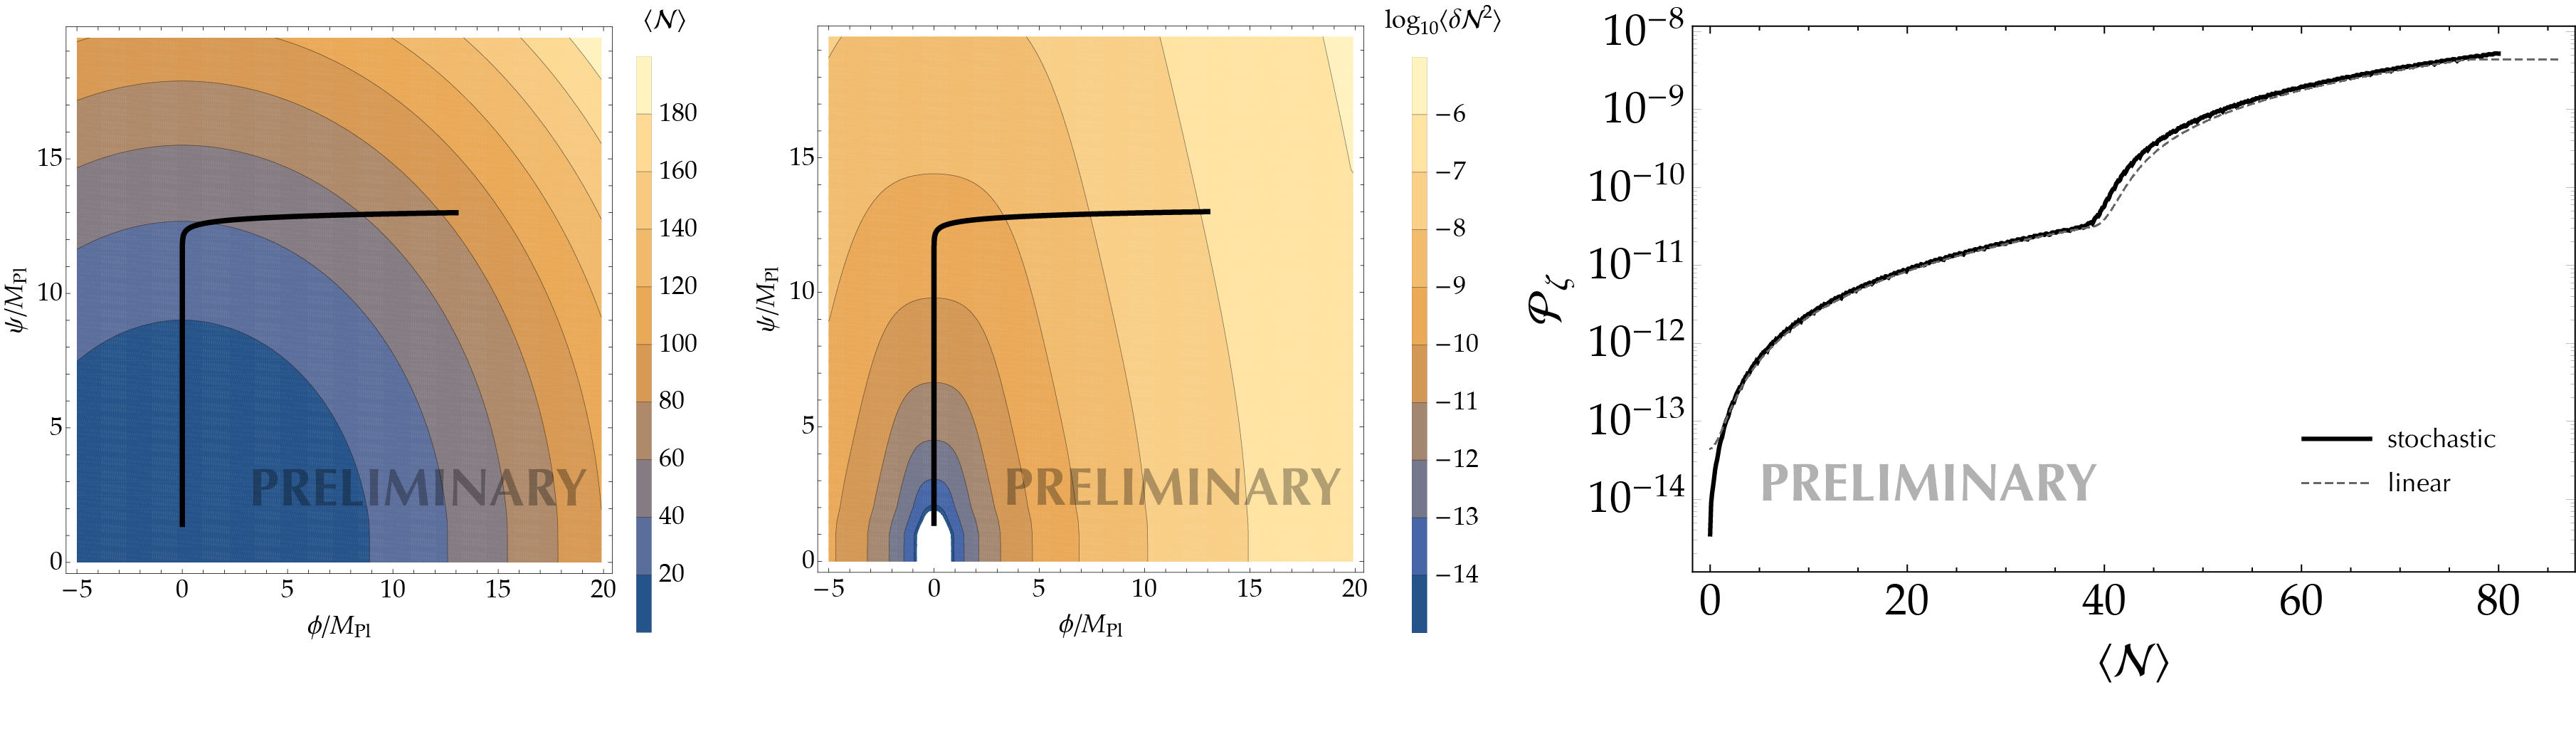
\includegraphics[width=\hsize]{figs/sample_plots.png}
	\caption{ストカスティック-$\delta N$形式における数値計算コードのサンプル図. 左2つはインフラトン場空間における, インフレーション持続時間 (e-folds $\mathcal{N}$) と
	そのゆらぎの等高線をそれぞれ示しており, 黒太線は実際のインフラトンの軌跡を表している. $\delta N$形式によれば e-folds のゆらぎはそのまま観測量としての曲率ゆらぎを与えるので,
	インフラトン軌跡上でスペクトル分解することで曲率ゆらぎのパワースペクトル $\mathcal{P}_\zeta$ が求まり, それが右図に示されている.
	また左図に示されているようにインフラトン軌跡と e-folds 等高線が直交していない場合, 曲率ゆらぎが非ガウス性を持つことになり~\cite{Tada:2016pmk}, 
	我々の手法によって単にゆらぎの大きさだけでなくその統計性も解析されうることを示唆している.}
	\label{fig: StocDeltaN}
\end{figure}


\begin{mdframed}[roundcorner=0.5zw,
	%skipabove=1zw,skipbelow=1zw,
	innertopmargin=0.8zw,innerbottommargin=0.8zw,
	%innerleftmargin=0.8zw,innerrightmargin=0.8zw,
	%rightmargin=5000pt,leftmargin=50pt,
	linecolor=black!50,linewidth=0.2zw,
	backgroundcolor=black!10]
	{\bfseries\gtfamily\sffamily\large 2. 研究環境}
\end{mdframed}

数値計算に関して, 申請者が所属している名古屋大学宇宙論研究室ではクラスタコンピュータ ``galaxy" を所有しており, 計算コード開発に大いに役立っている.
PC も特別研究員奨励費を利用して新調することができたので, コード開発に全く支障はない.
人材面に関しては, 共同研究者の一人である\emph{徳田}氏は京都大学所属であり名古屋大学からそう遠くない. また今夏から同研究室配属となった\emph{横山}氏は
$\delta N$形式に精通しており, 以前宇宙線研究所において共同研究した経験~\cite{Tada:2015noa}もあることから, 現在の研究においても有意義な意見を
いただいている. 同様に宇宙線研究所出身で, 現在共に名古屋大学で PD 特別研究員として働いている\emph{北嶋}氏も, ストカスティック形式を研究に用いた経験があり心強い. 
他にも名古屋大学にはストカスティック形式の大家である\emph{南部}氏や PBH 形成に詳しい\emph{柳}氏など豊富な人材が揃っており, 本研究の遂行に適した環境であると言える.
共同研究者である \emph{Renaux-Petel} 氏や \emph{Vennin} 氏がいるフランスとは離れているが, 普段はメールや Skype を利用したり, あるいは特別研究員奨励費を
利用してフランスを訪問したりすることで研究を行なっている.
ただしよりスムーズな研究遂行のためには, 彼らとのさらなる交流や他の海外研究者 (例えばイギリス Institute of Cosmology and Gravitation の \emph{Wands} 氏や 
ICL の \emph{Tolley} 氏, 
ユトレヒト大学の \emph{Prokopec} 氏らに
興味を持っていただいている) との議論のため本科研費が必要不可欠であると考える.


\vspace{1cm}
\begin{thebibliography}{99}
\bibitem{Tada:2016pmk} 
  \me and V.~Vennin,
  %``Squeezed bispectrum in the $\delta N$ formalism: local observer effect in field space,''
  JCAP {\bf 1702}, no. 02, 021 (2017)
  %doi:10.1088/1475-7516/2017/02/021
  %[arXiv:1609.08876 [astro-ph.CO]].
  %%CITATION = doi:10.1088/1475-7516/2017/02/021;%%
  %6 citations counted in INSPIRE as of 18 Oct 2018
  
  \bibitem{Kawasaki:2016pql} 
  M.~Kawasaki, A.~Kusenko, \me and T.~T.~Yanagida,
  %``Primordial black holes as dark matter in supergravity inflation models,''
  Phys.\ Rev.\ D {\bf 94}, no. 8, 083523 (2016)
  %doi:10.1103/PhysRevD.94.083523
  %[arXiv:1606.07631 [astro-ph.CO]].
  %%CITATION = doi:10.1103/PhysRevD.94.083523;%%
  %49 citations counted in INSPIRE as of 30 Oct 2018
  
  \bibitem{Inomata:2016rbd} 
  K.~Inomata, M.~Kawasaki, K.~Mukaida, \me and T.~T.~Yanagida,
  %``Inflationary primordial black holes for the LIGO gravitational wave events and pulsar timing array experiments,''
  Phys.\ Rev.\ D {\bf 95}, no. 12, 123510 (2017)
  %doi:10.1103/PhysRevD.95.123510
  %[arXiv:1611.06130 [astro-ph.CO]].
  %%CITATION = doi:10.1103/PhysRevD.95.123510;%%
  %44 citations counted in INSPIRE as of 30 Oct 2018
  
  \bibitem{Tada:2015noa} 
  \me and S.~Yokoyama,
  %``Primordial black holes as biased tracers,''
  Phys.\ Rev.\ D {\bf 91}, no. 12, 123534 (2015)
  %doi:10.1103/PhysRevD.91.123534
  %[arXiv:1502.01124 [astro-ph.CO]].
  %%CITATION = doi:10.1103/PhysRevD.91.123534;%%
  %20 citations counted in INSPIRE as of 18 Oct 2018
  
  \bibitem{Fujita:2015iga} 
  T.~Fujita, R.~Namba, \me, N.~Takeda and H.~Tashiro,
  %``Consistent generation of magnetic fields in axion inflation models,''
  JCAP {\bf 1505}, no. 05, 054 (2015)
  %doi:10.1088/1475-7516/2015/05/054
  %[arXiv:1503.05802 [astro-ph.CO]].
  %%CITATION = doi:10.1088/1475-7516/2015/05/054;%%
  %42 citations counted in INSPIRE as of 30 Oct 2018
  
  \bibitem{Inomata:2016uip} 
  K.~Inomata, M.~Kawasaki and \me,
  %``Revisiting constraints on small scale perturbations from big-bang nucleosynthesis,''
  Phys.\ Rev.\ D {\bf 94}, no. 4, 043527 (2016)
  %doi:10.1103/PhysRevD.94.043527
  %[arXiv:1605.04646 [astro-ph.CO]].
  %%CITATION = doi:10.1103/PhysRevD.94.043527;%%
  %11 citations counted in INSPIRE as of 30 Oct 2018
  
  \bibitem{Fujita:2013cna-2} 
  T.~Fujita, M.~Kawasaki, \me and T.~Takesako,
  %``A new algorithm for calculating the curvature perturbations in stochastic inflation,''
  JCAP {\bf 1312}, 036 (2013)
  %doi:10.1088/1475-7516/2013/12/036
  %[arXiv:1308.4754 [astro-ph.CO]].
  %%CITATION = doi:10.1088/1475-7516/2013/12/036;%%
  %17 citations counted in INSPIRE as of 18 Oct 2018
  
  \bibitem{Fujita:2014tja} 
  T.~Fujita, M.~Kawasaki and \me,
  %``Non-perturbative approach for curvature perturbations in stochastic $\delta N$ formalism,''
  JCAP {\bf 1410}, no. 10, 030 (2014)
  %doi:10.1088/1475-7516/2014/10/030
  %[arXiv:1405.2187 [astro-ph.CO]].
  %%CITATION = doi:10.1088/1475-7516/2014/10/030;%%
  %18 citations counted in INSPIRE as of 18 Oct 2018
  
  \bibitem{Kawasaki:2015ppx-2} 
  M.~Kawasaki and \me,
  %``Can massive primordial black holes be produced in mild waterfall hybrid inflation?,''
  JCAP {\bf 1608}, no. 08, 041 (2016)
  %doi:10.1088/1475-7516/2016/08/041
  %[arXiv:1512.03515 [astro-ph.CO]].
  %%CITATION = doi:10.1088/1475-7516/2016/08/041;%%
  %19 citations counted in INSPIRE as of 18 Oct 2018
  
  \bibitem{Pinol:2018euk-2} 
  L.~Pinol, S.~Renaux-Petel and \me,
  %``A critical look at stochastic inflation,''
  arXiv:1806.10126 [gr-qc].
  %%CITATION = ARXIV:1806.10126;%%
\end{thebibliography}


\begin{comment}
	応募者は過去20年間、7つの海を隅から隅まで航海し、
	浅瀬から深海まで潜り、文字通り東西南北上下の3次元で
	シロナガスクジラの卵の探索を行ってきた(業績\ref{pub:whale})。
	シロナガスクジラに飲み込まれそうになったり、海賊に捕まるなどの危険な目にも
	あったが、それにもめげず、研究を遂行してきた強靭な能力を有する。

	シロナガスクジラの卵を探すために用いていたソナーと双眼鏡、及び
	シロナガスクジラの卵を引き上げるために用意していた大きな網は、
	そのまま使える。
\end{comment}
%end 応募者の研究遂行能力及び研究環境 ====================
%begin 研究業績リスト ====================
\begin{comment}
	\begin{enumerate}
		\item \label{pub:whale} ``Search for whale eggs'', 
				\me\ {\it et al.},
				Rev. Oceanic Mysteries, {\bf 888}, 99 (2017).
				
		\item \label{pub:theoegg} ``Theory of Elephant Eggs'', 
				\me, \underline{Kara Juzo}, {\it et al.},
				Phys.\ Rev.\ Lett. {\bf 800}, 800-804 (2005). 
				
		\item ``仔象は死んだ'', 
				\underline{Kobo Abe}, 
				安部公房全集, {\bf 26}, 100-200 (2004).
		\item ``The Elephant's Child (象の鼻はなぜ長い)'', 
				\underline{R.~Kipling},
				Nature, {\bf 999}, 777-779 (2003).
		\item ``You can't Lay an Egg If You're an Elephant'', 
				\underline{F.~Ehrlich},
				JofUR\\
				 ({\tt www.universalrejection.org}), {\bf N/A}, N/A (2002).
		\item ``Egg of Elephant-Bird'', 
				\underline{A.~Cooper},
				Nature, {\bf 409}, 704-707 (2001).	
			\item Jack Torrance, ``All work and no play makes Jack a dull boy", The Shining (1980).
	\item \hspace{5mm}Jack Torrance, '`All work and no play makes Jack a dull boy", The Shining (1980).
	\item \hspace{10mm}Jack Torrance, ``All work and no play makes Jack a dull boy", The Shining (1980).
	\item \hspace{15mm}Jack Torrance, ``All work and no play makes Jack a dull boy", The Shining (1980).
	\item \hspace{20mm}Jack Torrance, ``All work and no play makes Jack a dull boy", The Shining (1980).
	\item \hspace{25mm}Jack Torrance, ``All work and no play makes Jack a dull boy", The Shining (1980).
	\item \hspace{30mm}Jack Torrance, ``All work and no play makes Jack a dull boy", The Shining (1980).
	\item \hspace{25mm}Jack Torrance, ``All work and no play makes Jack a dull boy", The Shining (1980).
	\item \hspace{20mm}Jack Torrance, ``All work and no play makes Jack a dull boy", The Shining (1980).
	\item \hspace{15mm}Jack Torrance, ``All work and no play makes Jack a dull boy", The Shining (1980).
	\item \hspace{10mm}Jack Torrance, ``All work and no play makes Jack a dull boy", The Shining (1980).
	\item \hspace{5mm}Jack Torrance, ``All work and no play makes Jack a dull boy", The Shining (1980).
	\item Jack Torrance, ``All work and no play makes Jack a dull boy", The Shining (1980).
	% << only for demonstration. Please delete it or comment it out.
	\end{enumerate}
\end{comment}
%end 研究業績リスト ====================

% p03_abilities_01.tex
\KLEndSubject{F}


%#Split: 05_rights  
%#PieceName: p05_rights
% p05_rights_00.tex
\KLBeginSubject{04}{4}{4 人権の保護及び法令等の遵守への対応}{1}{F}{}{jsps-subject-header}{jsps-default-header}

\section{4 人権の保護及び法令等の遵守への対応}
%    <<最大 1ページ>>

% s09_rights
%begin 人権の保護及び法令等の遵守への対応 ====================
	該当しない.
%end 人権の保護及び法令等の遵守への対応 ====================

% p05_rights_01.tex
\KLEndSubject{F}


%#Split: 99_tail
% hook9 : right before \end{document} ============
 % pieces
\end{document}
